\section{Maze and multi-agent exploration}
\label{section_models_maze}
For simulation purposes, this work modeled a maze under an interrelated cells perspective, where each cell is a square with its edges composed by a wall or not. If there is a wall, an agent cannot traverse the maze across the related edge. On the other hand, if there is not a wall, an agent has a free way to traverse the maze through the related edge. It is worth to mention that, if an edge has a wall, the edge of the adjacent corresponding cell also has necessarily a wall.

The maze has a goal that is a single marked cell, and an agent inside the maze aims to find the marked cell, traversing the maze cell by cell. This agent is an autonomous entity that follows a specific algorithm according the current explored path and its programmed initial rules. So that it doesn't go through the same path more than one time, it stores the visited cells. Thus, every time the agent find a branched cell (a cell with at least one edge without a wall), it ignores the already visited branches by itself, and, if there is not a candidate to be a possible branch, the agent go back to the previous visited cell. Furthermore, specifically to this research, differently from some approaches presented in \citen{Beisel2014}, \citen{Burgard2005}, and \citen{KivelevitchCohen2010}, there is no intercommunication between agents in a multi-agent situation to solve the maze.

\citen{Muhammad2021} developed an open-source maze generator. It is a python module that creates randomly mazes and enables the user to simulate its own maze-solving algorithm. In this context, this work presents a multi-agent maze-solving algorithm that has been simulated over \citen{Muhammad2021} open-source code, with modifications. The Figure \ref{maze_model} presents, for example, 2 agents traversing a $6 \times 6$ maze toward the goal.

\citen{Muhammad2021} software creates by default a ``perfect maze'', which means that there is one and only one path to the goal from any cell. However, it is possible to set the code to generate a imperfect maze.

\begin{figure}[ht!]
\centering
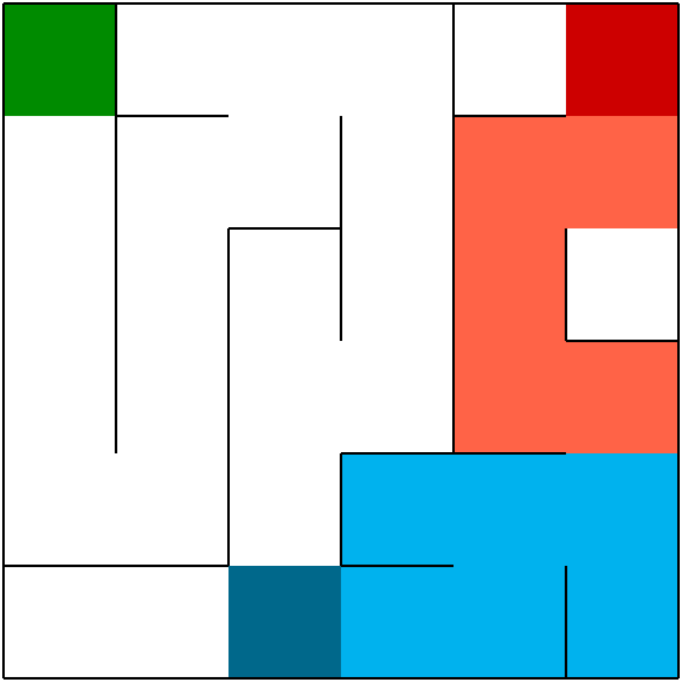
\includegraphics[width=0.5\textwidth]{Cap2/maze_model.png}
\caption{Blue and red agents traversing a $6\times 6$ maze. The goal is represented by the green entity. This maze is a perfect maze \cite{Muhammad2021}.}
\label{maze_model}
\end{figure}

\section{Maze from a graph topology perspective}
\label{section_models_maze_graph}
As pointed out in Section \ref{section_models_maze}, given that an agent ignores visited cells, there are important statements related to this work:

\begin{itemize}
\item if there is only one path to the goal from any cell, it is valid to consider a maze as a tree, i.e., a perfect maze \cite{Muhammad2021};

\item if there is more than one path to the goal from any cell, the maze cannot be considered as a tree, but it might be considered as a graph;

\item despite the last statement, and also considering that an agent ignores visited cells, an agent path always might be individually interpreted as a tree.
\end{itemize}

Figure \ref{maze_example_graph} gives an example of the graph representation of the maze presented in Figure \ref{maze_example}, where a red agent is traversing the maze toward the green goal. As established by \citen{Muhammad2021}, the maze cells are programmatically addressed as indices of a matrix, such as represented in Figure \ref{maze_indices_muhammad}.

\begin{figure}[ht!]
\centering
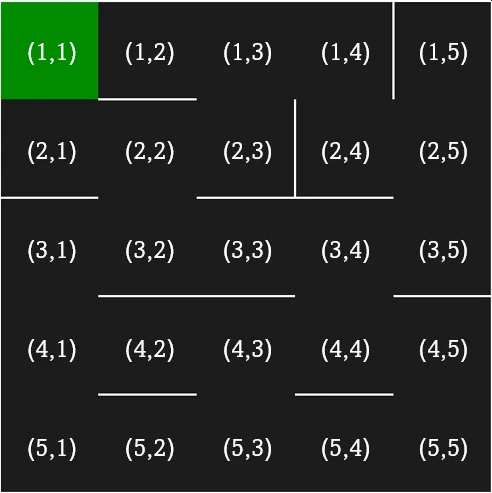
\includegraphics[width=0.5\textwidth]{Cap2/maze_indices_muhammad.png}
\caption{Maze cell indices. Source: \citen{Muhammad2021}.}
\label{maze_indices_muhammad}
\end{figure}

\begin{figure}[ht!]
\centering
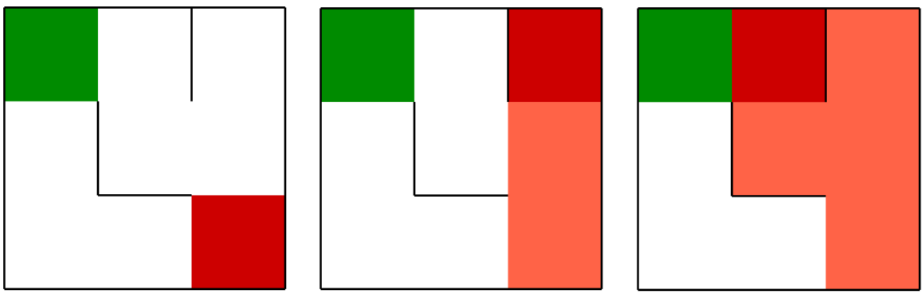
\includegraphics[width=0.7\textwidth]{Cap2/maze_example.png}
\caption{Red agent traversing a maze toward the green goal. This maze is not a perfect maze.}
\label{maze_example}
\end{figure}

\begin{figure}[ht!]
\centering
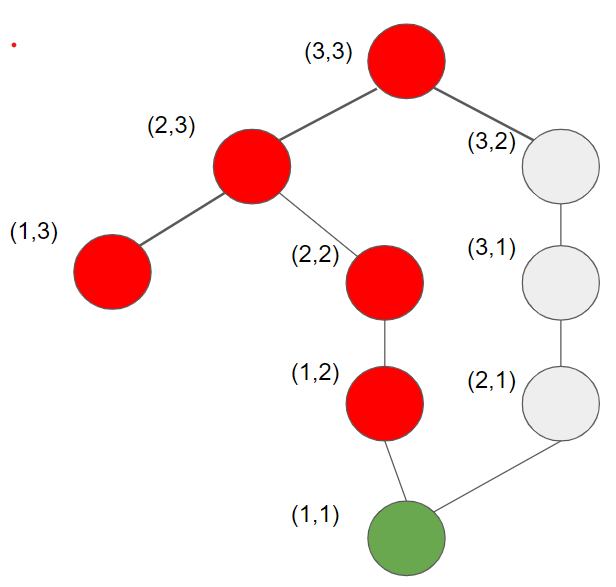
\includegraphics[width=0.5\textwidth]{Cap2/maze_example_graph.png}
\caption{Graph representation of the maze presented in Figure \ref{maze_example}. The cell indices are pointed out. Furthermore, the visited cells by the red agent are also pointed out.}
\label{maze_example_graph}
\end{figure}	

\section{Multi-agent exploration without communication}
\label{section_models_mixed_radix}
The goal of this work is to present a maze-solving algorithm in a multi-agent environment, where an agent cannot communicate with the other agents. Thus, each agent must be previously programmed to avoid traversing the maze through the same way related to another agent.

First of all, this research considers a maze as a graph, where each node is a cell representation of the maze. Given a initial node that the agent starts its path through it, the agent checks if the node has children. Supposing that a node of the graph has at least one child, i.e., there are not completely walled cells, important statements are established:

\begin{itemize}
\item if an agent finds the node where is the goal, the agent finishes its path;

\item if an agent is not in the node where is the goal and the node has only one child, the agent necessarily goes through this node child;

\item if an agent is not in the node where is the goal and the node has more than one child, the agent needs to make a decision about which child to choose;
\end{itemize}

To establish an decision algorithm to the last statement, this work proposes firstly a interval division related to the agents and the children. Supposing that there are $n$ agents $a_{1}, a_{2},...,a_{n}$ to explore the maze, each agent will have a corresponding and proportional range of action related to the graph, as presented below:

\begin{equation}
	\begin{align}
			d = 1/n\\
		a_{1} \textnormal{: } [0, d[\\
		a_{2} \textnormal{: } [d, 2d[\\
		a_{3} \textnormal{: } [3d, 4d[\\
		...\\
		a_{n} \textnormal{: } [(n-1)d, 1]
	\end{align}
\end{equation}
where $d$ it the size of the partition corresponding to each agent.

On the other hand, this work has been handled corresponding intervals to each child of a node, as presented in Figure \ref{maze_example_graph_intervals}, that represents the maze in Figure \ref{maze_example}. Thus, the goal of this work aims to establish an efficient algorithm that interrelates the agent intervals to the graph intervals. Furthermore, a mixed radix representation to the agent path has been studied.

\begin{figure}[ht!]
\centering
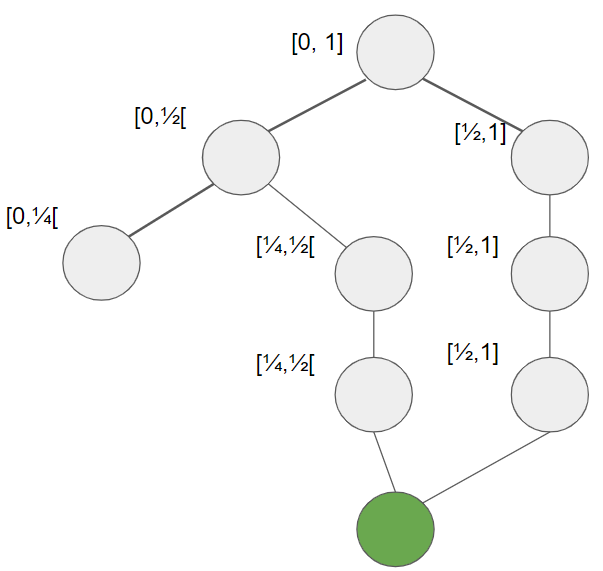
\includegraphics[width=0.5\textwidth]{Cap2/maze_example_graph_intervals.png}
\caption{Graph representation of the maze presented in Figure \ref{maze_example}, with intervals related to the agent's range of action.}
\label{maze_example_graph_intervals}
\end{figure}	